\documentclass[12pt,a4paper]{article}
\usepackage{cmap} % Makes the PDF copiable. See http://tex.stackexchange.com/a/64198/25761
\usepackage[T1]{fontenc}
\usepackage[brazil]{babel}
\usepackage[utf8]{inputenc}
\usepackage{amsmath}
\usepackage{amsfonts}
\usepackage{amssymb}
\usepackage{amsthm}
\usepackage{textcomp} % \degree
\usepackage{gensymb} % \degree
\usepackage[usenames,svgnames,dvipsnames]{xcolor}
\usepackage{hyperref}
\usepackage{graphicx}
\usepackage[margin=2cm]{geometry}

\hypersetup{
    colorlinks = true,
    allcolors = {blue}
}

% TODO: Consider using exsheets
% http://linorg.usp.br/CTAN/macros/latex/contrib/exsheets/exsheets_en.pdf
%
% http://ctan.org/tex-archive/macros/latex/contrib/exercise/
% Options: answerdelayed,lastexercise,noanswer
\usepackage[answerdelayed,lastexercise]{exercise}

\addto\captionsbrazil{%
\def\listexercisename{Lista de exerc\'icios}%
\def\ExerciseName{Exerc\'icio}%
\def\AnswerName{Solu\c{c}\~ao do exerc\'icio}%
\def\ExerciseListName{Ex.}%
\def\AnswerListName{Solu\c{c}\~ao}%
\def\ExePartName{Parte}%
\def\ArticleOf{de\ }%
}

\renewcommand{\ExerciseHeaderTitle}{(\ExerciseTitle)\ }
\renewcommand{\ExerciseListHeader}{%\ExerciseHeaderDifficulty%
\textbf{%\ExerciseListName\
\ExerciseHeaderNB.\ %
%\ --- \ 
\ExerciseHeaderTitle}%
%\ExerciseHeaderOrigin
\ignorespaces}
\renewcommand{\AnswerListHeader}{\textbf{\ExerciseHeaderNB.\ (\AnswerListName)\ }}

\newcommand*\R{\mathbb{R}}
\newcommand{\vect}[1]{\overrightarrow{#1}}
\newcommand{\norm}[1]{\left|\left|{#1}\right|\right|}

\renewcommand{\theenumi}{\alph{enumi}}
\renewcommand\labelenumi{(\theenumi) }

\newcommand*\tipo{Prova I}
\newcommand*\turma{PRO112-01U}
\newcommand*\disciplina{GAN0001}
\newcommand*\eu{Helder G. G. de Lima}
\newcommand*\data{30/08/2016}

\author{\eu}
\title{\tipo - \disciplina}
\date{\data}

\begin{document}
\thispagestyle{empty}
\newgeometry{margin=2cm,bottom=0.5cm}
\begin{center}

\includegraphics[width=9.0cm]{marca} \\
\textbf{\tipo\ (\disciplina / \turma)} \\
Prof. \eu\footnote{
Este é um material de acesso livre distribuído sob os termos da licença \href{https://creativecommons.org/licenses/by-sa/4.0/deed.pt_BR}{Creative Commons BY-SA 4.0}.}
\end{center}

\noindent Nome do(a) aluno(a): \underline{\hspace{9,7cm}} Data: \underline{\data}

%\section*{Instruções}
\begin{center}\fbox{
\begin{minipage}{14cm}

{\footnotesize
\begin{itemize}
\renewcommand{\theenumi}{\Roman{enumi}}
\item Identifique-se em todas as folhas.
\item Mantenha o celular e os demais equipamentos eletrônicos desligados durante a prova.
\item Anule \textsc{\textbf{uma}} das questões (apenas 4 serão corrigidas): \framebox(30,10){}
\end{itemize}
}

\end{minipage}
}
\end{center}

%\section*{Questões}
\begin{ExerciseList}
\Exercise[title={2,5}] Sabendo que os lados de um triângulo equilátero $ABC$ têm comprimento $4$, calcule $\vect{AB}\cdot\vect{BC} + \vect{BC}\cdot\vect{CA} + \vect{CA}\cdot\vect{AB}$.
\Answer Os vetores dados podem ser representados como na seguinte figura:

\parbox{.7\linewidth}{%
Então, se $\alpha$, $\beta$ e $\gamma$ são os ângulos entre $\vect{AB}$ e $\vect{BC}$, $\vect{BC}$ e $\vect{CA}$ e $\vect{CA}$ e $\vect{AB}$, respectivamente:
\begin{itemize}
\item $\vect{AB}\cdot\vect{BC}
= \norm{ \vect{AB} } \cdot \norm{ \vect{BC} } \cos( \alpha)
= 4 \cdot 4 \cdot\left( \frac{-1}{2} \right) = -8$
\item $\vect{BC}\cdot\vect{CA}
= \norm{ \vect{BC} } \cdot \norm{ \vect{CA} } \cos( \beta)
= 4 \cdot 4 \cdot\left( \frac{-1}{2} \right) = -8$
\item $\vect{CA}\cdot\vect{AB}
= \norm{ \vect{CA} } \cdot \norm{ \vect{AB} } \cos( \gamma)
= 4 \cdot 4 \cdot\left( \frac{-1}{2} \right) = -8$
\end{itemize}
}
\parbox{.2\linewidth}{%
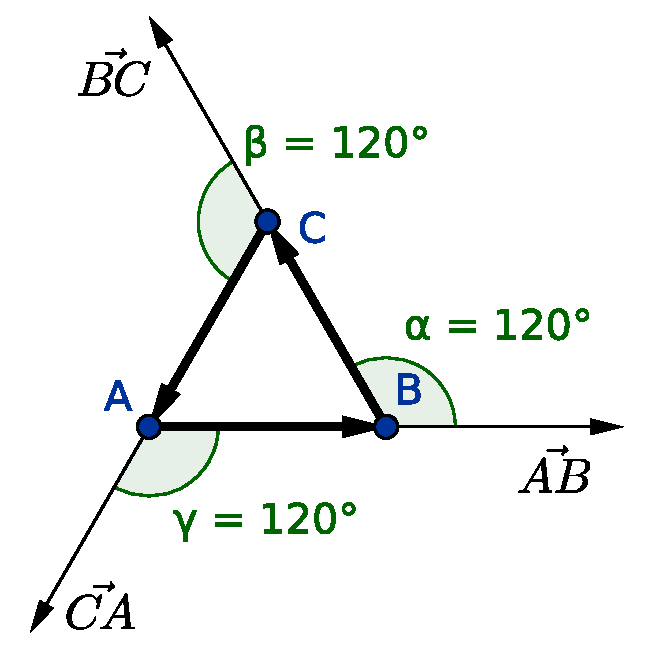
\includegraphics[width=5.0cm]{img/prova-1-pro-tri-equi}
}

Portanto, $\vect{AB}\cdot\vect{BC} + \vect{BC}\cdot\vect{CA} + \vect{CA}\cdot\vect{AB} = 3 \times (-8) = -24$.

\Exercise[title={2,5}] Sejam $A(1,-1,4)$, $B(-1,4,-3)$ e $C(0,0,1)$.
\begin{enumerate}
\item \textbf{(1,0)} Obtenha a área do triângulo com vértices $A$, $B$ e $C$.
\item \textbf{(1,5)} Determine $t \in \R$ para que $A$, $B$, $C$ e $D(6t-2, 2, 2t+2)$ sejam coplanares.
\end{enumerate}
\Answer
\begin{enumerate}
\item A área $A_{\Delta ABC}$ do triângulo com vértices $A$, $B$ e $C$ é a metade da área do paralelogramo determinado por estes pontos, que é $\norm{ \vect{AB} \times \vect{AC} }$. Mas
\[
\vect{AB} \times \vect{AC}
= \begin{vmatrix}
\vec{i} & \vec{j} & \vec{k} \\
-2 & 5 & -7 \\
-1 & 1 & -3
\end{vmatrix}
= -8 \vec{i} + \vec{j} -3 \vec{k}
= (-8, 1, -3),
\]
então $A_{\Delta ABC} = \frac{1}{2} \sqrt{ (-8)^2 + 1^2 + (-3)^2 } = \frac{\sqrt{74}}{2}$.

\item Os pontos $A$, $B$, $C$ e $D$ são coplanares quando o produto misto entre os vetores $\vect{AB}$, $\vect{AC}$ e $\vect{AD}$ é zero. Mas $\vect{AB} = (-2,5,-7)$, $\vect{AC} = (-1,1,-3)$ e $\vect{AD}=(6t-3, 3, 2t-2)$, então
\[
[ \vect{AB}, \vect{AC}, \vect{AD} ]
=
\begin{vmatrix}
-2 & 5 & -7\\
-1 & 1 & -3\\
6t-3 & 3 & 2t-2
\end{vmatrix}
= -42t + 21.
\]
Assim, $[ \vect{AB}, \vect{AC}, \vect{AD} ] = 0$ se, e somente se, $t = \frac{21}{42} = \frac{1}{2}$.
\end{enumerate}

\Exercise[title={2,5}] Supondo que
$\vec{u} = \left(\frac{3}{2}, \frac{3}{2}, -2\right)$,
$\vec{v} = (0,2,2)$ e
$\vec{w} = (2,0,2)$, calcule:
\begin{enumerate}
\item \textbf{(1,0)} As coordenadas do vetor $\text{Proj}_{\vec{w}} \vec{v}$ (isto é, a projeção de $\vec{v}$ sobre $\vec{w}$).
\item \textbf{(1,5)} O ângulo que o vetor $\vec{d} = \vec{u} \times (\vec{v} \times \vec{w})$ forma com os vetores $\vec{v}$ e $\vec{w}$.
\end{enumerate} 
\Answer
\begin{enumerate}
\item $\text{Proj}_{\vec{w}} \vec{v}
= \left( \frac{\vec{v} \cdot \vec{w}}{ \norm{ \vec{w} }^2} \right) \vec{w}
= \left( \dfrac{ (0,2,2) \cdot (2,0,2) }{ \norm{ (2,0,2) }^2} \right) (2,0,2)
= \frac{ 4 }{ 8 } (2,0,2)
= (1,0,1)$.
\item Observe que $
\vec{d}
= \vec{u} \times ( \vec{v} \times \vec{w})
= \begin{vmatrix}
\vec{v}               &               \vec{w} \\
\vec{u} \cdot \vec{v} & \vec{u} \cdot \vec{w}
\end{vmatrix}
= \begin{vmatrix}
\vec{v} & \vec{w} \\
     -1 &      -1
\end{vmatrix}
= -\vec{v} + \vec{w} = (2,-2,0).
$
Então, se $\theta_1$ é o ângulo entre $\vec{d}$ e $\vec{v}$ e $\theta_2$ é o ângulo entre $\vec{d}$ e $\vec{w}$, resulta que
\begin{itemize}
\item $\cos( \theta_1 )
= \dfrac{ (2,-2,0) \cdot (0,2,2) }{ \norm{ (2,-2,0) } \cdot \norm{ (0,2,2) } }
= \dfrac{-4}{\sqrt{8} \sqrt{8} }
= \dfrac{-1}{2}$.
\item $\cos( \theta_2 )
= \dfrac{ (2,-2,0) \cdot (2,0,2) }{ \norm{ (2,-2,0) } \cdot  \norm{ (2,0,2) } }
= \dfrac{4}{\sqrt{8} \sqrt{8} }
= \dfrac{1}{2}$.
\end{itemize}
Portanto, $\theta_1 = \frac{2\pi}{3}$ e $\theta_2 = \frac{\pi}{3}$.
\end{enumerate} 

\Exercise[title={2,5}] Dados os pontos $P(1,-3,2)$, $Q(2a+1, 3, b + 5)$, $R(1,-2,5)$ e $S(4,-3,5)$, calcule:
\begin{enumerate}
\item \textbf{(1,5)} Os valores de $a$ e $b$, sabendo que $\vect{PQ}$ é simultaneamente ortogonal a $\vect{PR}$ e a $\vect{PS}$.
\item \textbf{(1,0)} O volume do tetraedro determinado pelos pontos indicados.
\end{enumerate} 
\Answer
\begin{enumerate}
\item Observe que
$\vect{PQ} = (2a, 6,b+3)$,
$\vect{PR} = (0,1,3)$ e
$\vect{PS} = (3,0,3)$, e que para $\vect{PQ}$ ser ortogonal tanto a $\vect{PR}$ quanto a $\vect{PS}$, deve ocorrer

\[
\begin{cases}
\vect{PQ} \cdot \vect{PR} & = 0\\
\vect{PQ} \cdot \vect{PS} & =0
\end{cases}
\Leftrightarrow
\begin{cases}
6 + 3b + 9 & = 0\\
6a + 3b + 9 & = 0
\end{cases}
\Leftrightarrow
\begin{cases}
3b & = -15\\
6a + 3b & = -9
\end{cases}
\]
Da primeira equação, resulta que $b = -5$, e substituindo este valor na segunda equação, conclui-se que $a = 1$. Em particular, tem-se $Q(3,3,0)$ e $\vect{PQ} = (2,6,-2)$.
\item O volume do tetraedro é um sexto do volume do paralelepípedo definido por $P$, $Q$ $R$ e $S$:
\[
V
= \frac{1}{6}
\left| [ \vect{PQ}, \vect{PR}, \vect{PS}] \right|
= \frac{1}{6} 
\left|\det
\begin{bmatrix}
2 & 6 & -2\\
0 & 1 &  3\\
3 & 0 &  3
\end{bmatrix}
\right|
=\frac{1}{6}| 6+54+6|
=\frac{66}{6}
=11
.
\]
\end{enumerate} 

\Exercise[title={2,5}] Determine as coordenadas de um vetor $\vec{v}$, que forme o mesmo ângulo (agudo) com os vetores $\vec{i}$, $\vec{j}$ e $\vec{k}$, e cuja projeção sobre o vetor $\vec{w} = (6,-3,6)$ tenha norma $4$.
\Answer Se os ângulos diretores de $\vec{v}$ são $\alpha$, $\beta$ e $\gamma$, então o fato de $\vec{v}$ formar o mesmo ângulo agudo com os três eixos implica que $\cos(\alpha) = \cos(\beta) = \cos(\gamma) > 0$. Assim, se $\vec{v} = (x,y,z)$, pode-se afirmar que $\frac{x}{\norm{v}} = \frac{y}{\norm{v}} = \frac{z}{\norm{v}} > 0$, ou seja, $x=y=z > 0$ e $\vec{v} = (x,x,x)$.

Por hipótese,
\[
4 = \norm{\text{Proj}_{(6,-3,6)} \vec{v}}
= \frac{ | (x,x,x) \cdot (6,-3,6) | }{ \norm{(6,-3,6)} }
= \frac{ |6x -3x + 6x| }{ \sqrt{ 36 + 9 + 36} }
= \frac{ 9|x| }{ 9 }
= |x|
\]
Como $x > 0$, conclui-se que $x = 4$ e $\vec{v} = (4,4,4)$.

\end{ExerciseList}

\begin{center}
BOA PROVA!
\end{center}

\newpage
\restoregeometry
\section*{Respostas}
\shipoutAnswer
\end{document}
